\let\negmedspace\undefined
\let\negthickspace\undefined
\documentclass[journal]{IEEEtran}
\usepackage[a5paper, margin=10mm, onecolumn]{geometry}
%\usepackage{lmodern} % Ensure lmodern is loaded for pdflatex
\usepackage{tfrupee} % Include tfrupee package

\setlength{\headheight}{1cm} % Set the height of the header box
\setlength{\headsep}{0mm}     % Set the distance between the header box and the top of the text

\usepackage{gvv-book}
\usepackage{gvv}
\usepackage{cite}
\usepackage{amsmath,amssymb,amsfonts,amsthm}
\usepackage{algorithmic}
\usepackage{graphicx}
\usepackage{textcomp}
\usepackage{xcolor}
\usepackage{txfonts}
\usepackage{listings}
\usepackage{enumitem}
\usepackage{mathtools}
\usepackage{gensymb}
\usepackage{comment}
\usepackage[breaklinks=true]{hyperref}
\usepackage{tkz-euclide} 
\usepackage{listings}
% \usepackage{gvv}                                        
\def\inputGnumericTable{}                                 
\usepackage[latin1]{inputenc}                                
\usepackage{color}                                            
\usepackage{array}                                            
\usepackage{longtable}                                       
\usepackage{calc}                                             
\usepackage{multirow}                                         
\usepackage{hhline}                                           
\usepackage{ifthen}                                           
\usepackage{lscape}
\begin{document}
\bibliographystyle{IEEEtran}
\title{3.3.20}
\author{EE24BTECH11007 - Arnav Makarand Yadnopavit}
{\let\newpage\relax\maketitle}
\renewcommand{\thefigure}{\theenumi}
\renewcommand{\thetable}{\theenumi}
\setlength{\intextsep}{10pt} % Space between text and floats
\numberwithin{equation}{enumi}
\numberwithin{figure}{enumi}
\renewcommand{\thetable}{\theenumi}
\parindent 0px
Question:\\
Draw a triangle ABC in which AB=5 cm, BC=6 cm and $\angle$ ABC = 60$\degree$.Then construct a triangle whose sides are $\frac{5}{7}$ times the corresponding sides of $\triangle$ABC.\\
\solution
\begin{table}[h]
    \centering
    \begin{tabular}{|c|p{3cm}|p{3cm}|}
    \hline
    Symbol & Description & Value\\
    \hline
    $a$ & length of side BC & 6 cm\\
    \hline
    $b$ & length of side CA & $b$\\
    \hline
    $c$ & length of side AB & 5 cm\\
    \hline
    $a_0$ & length of side BC of second triangle & $a_0$\\
    \hline
    $b_0$ & length of side CA of second triangle & $b_0$\\
    \hline
    $c_0$ & length of side AB of second triangle & $c_0$\\
    \hline
    $\angle B$ & angle at vertex B & 60$\degree$\\
    \hline
\end{tabular}
    \caption{Given Values}
    \label{tab:1}
\end{table}\\
Using cosine rule
\begin{align}
\cos\brak{\angle B}=\frac{a^2+c^2-b^2}{2ac}\\
\implies b=\sqrt{31}
\end{align}
As sides of second triangle are $\frac{5}{7}$ times the corresponding sides of $\triangle$ABC.
\begin{align}
	a_0&=\frac{30}{7}cm\\
	b_0&=\frac{25}{7}cm\\
	c_0&=\frac{5\sqrt{31}}{7}cm
\end{align}

\begin{figure}[h]
    \centering
    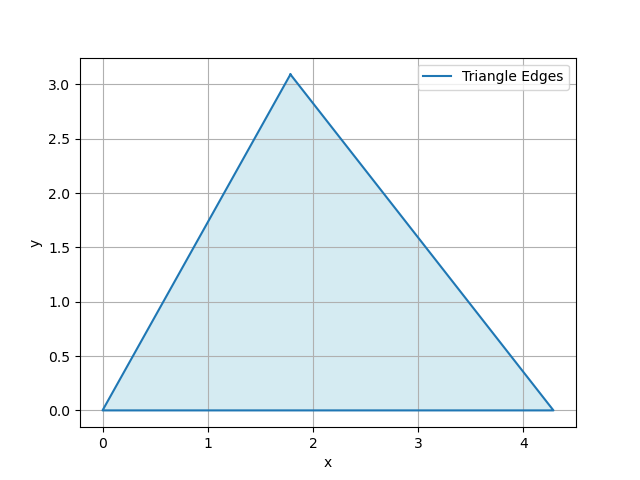
\includegraphics[width=\columnwidth]{figs/fig.png}
    \caption{Plot of $\triangle$A'BC' and $\triangle$ABC}
 \end{figure}
\end{document}
